\documentclass[10pt,a4paper]{article}
\usepackage[latin1]{inputenc}
\usepackage{amsmath}
\usepackage{amsfonts}
\usepackage{amssymb}
\usepackage{graphicx}
\author{Connor Noyes}
\title{Stochastic Entry Guidance}
\begin{document}
	\maketitle
%	\section{EoM}
%		The 3DOF equations of motion are
%		\begin{align}
%		& \dot{h} = V\sin\gamma \\
%		& \dot{\theta} = \dfrac{V\cos\gamma}{r}\dfrac{\cos\psi}{\cos\phi} \\
%		& \dot{\phi} = \dfrac{V\cos\gamma}{r}\sin\psi \\
%		& \dot{V} = -D-g\sin\gamma \\
%		& \dot{\gamma} = \dfrac{L}{V}\cos\sigma - (g/V-V/r)\cos\gamma \\
%		& \dot{\psi} = \dfrac{L\sin\sigma}{V\cos\gamma}
%		\end{align}
%		
%		The methods employed here must use a fixed final independent value, so either energy, velocity, or trajectory length may be used in place of time. The 3DOF equations of motion with respect to energy are 
%		\begin{align}
%		& h' = -\frac{\sin\gamma}{D} \\
%		& \theta' = -\dfrac{\cos\gamma}{rD}\dfrac{\cos\psi}{\cos\phi} \\
%		& \phi' = -\dfrac{\cos\gamma}{rD}\sin\psi \\
%		& \gamma' = -\dfrac{L}{V^2D}\cos\sigma + (g/V-V/r)\dfrac{\cos\gamma}{VD} \\
%		& \psi' = -\dfrac{L\sin\sigma}{V^2D\cos\gamma} \\
%		& V = f(E,h) = \sqrt{2(E+\dfrac{\mu}{h+r_p})}
%		\end{align}
%		and the longitudinal equations with respect to energy are the reduced set
%		\begin{align}
%		& h' = -\frac{\sin\gamma}{D} \\
%		& s' = -\dfrac{\cos\gamma}{D} \\
%		& \gamma' = -\dfrac{L}{V^2D}u + (g/V-V/r)\dfrac{\cos\gamma}{VD} \\
%		& V = f(E,h) = \sqrt{2(E+\dfrac{\mu}{h+r_p})}
%		\end{align}
		
%	\section{Problem Statement}

%		Outline: Pose the stochastic problem. 
% Show that to first order, the trajectory of mean parameters is the mean trajectory. Second order effects take into account covariance. Thus, we can assume the nominal trajectory determines the mean trajectory, and closed-loop guidance controls the variance. Then, nominal trajectory is continually redesigned via sensitivity method (possibly framed as a mean/covariance argument again), and the loop is closed using feedback linearization (likely using an observer, potentially extended to account for control saturation), showing that minimization of expected errors is a variance minimization problem.

%		The equations of motion governing the vehicle during entry are given by the affine-in-control $\mathrm{It\hat{o}}$ stochastic differential state equation (with respect to energy) and stochastic observation equation
%		\begin{align}
%		&dx = (f(x)+g(x)u)dE + F(x,u)d\omega \label{eq_ito_dynamics}\\
%		&y = h(x) + H(x)d\zeta
%		\end{align}
%		where $\omega,\;\zeta$ are Wiener processes with covariances \textbf{TODO: finish this}. The general entry guidance problem may be posed as finding the control, here taken to be the bank angle profile, that guides an entry vehicle subject to the dynamics in Eq.~(\ref{eq_ito_dynamics}) to some final condition $x(E_f)\in\Omega$. The final condition is very general and has as special cases fully- or partially-specified final states, a target set defined by, e.g., conditions for parachute deployment or supersonic retropropulsion ignition, and optimal control problems where $\Omega$ is defined by an extremal quantity such as maximum crossrange subject to a minimum terminal altitude.
%		
%		The presence of significant uncertainty in the form of initial conditions, system parameters, or process/measurement noise leads to a desire to control not individual trajectories but families of trajectories forming a distribution. In the stochastic setting, Kolmogorov's Forward equation (also referred to as the Fokker-Planck equation)
%		\begin{equation}
%		\dfrac{\partial \mu}{\partial t} = -\mathrm{trace}\left(\dfrac{\partial f}{\partial x} + g(x)\dfrac{\partial u}{\partial x}\right)\mu+ \dfrac{\partial^2 f}{\partial x^2} \label{eq_kolmogorov_forward}
%		\end{equation}
%		governs the evolution of the distribution $\mu(t,x)$. If the Brownian motion term $F(x,u)=0$, the problem becomes deterministic (but still uncertain) and Eq.~(\ref{eq_kolmogorov_forward}) reduces to the Liouville equation
%		\begin{equation}
%		\dfrac{\partial \mu}{\partial t} = -\mathrm{trace}\left(\dfrac{\partial f}{\partial x} + g(x)\dfrac{\partial u}{\partial x}\right)\mu = -\mathrm{div}(f(x)+g(x)u(t,x))\mu. \label{eq_liouville}
%		\end{equation}

	\section{Motivation and Background}
%	Mease advice: give a bird's eye view of the problem. Show the current approach (MSL, linearized range control, separate lateral control, heading alignment) and discuss our approach and how it differs (near-optimal reference trajectories, combined range/lateral control, improved heading alignment, OUU). Can also discuss different UQ options in the loop (STM, QMC, PCE). 
% Pose the full problem, then state how MSL tackled it (and any assumptions), then give our approach (whatever that is...). Then give details, and results.

	Broadly speaking, the goal of entry, descent, and landing is to deliver a spacecraft safely to the planet surface. The modern era of Mars EDL, beginning with MSL in 2012, utilizes hypersonic entry guidance to reduce the landing footprint and deliver ever-increasing payload mass. The initial state of the vehicle at entry interface will differ from the planned entry state (delivery error), and this state will not be known exactly onboard the vehicle (knowledge error). Additionally, the models used in development of the onboard GNC system (such as the planetary atmosphere and the aerodynamics of the vehicle) are imperfect due to both inaccuracy in the model's parameters as well as the existence of unmodeled (or incorrectly modeled) dynamics.
	
	The Mars Science Laboratory spacecraft demonstrated the first guided entry on Mars when it landed in Gale Crater on August $5^{th}$, 2012. The vehicle flew with an offset center of mass to create an angle of attack that allowed the spacecraft to generate lift. The guidance approach used bank angle commands to orient the resulting lift vector and thereby compensate for dispersions.\cite{MSL_EDL_Overview_JPL}
	
	\subsection{Reference Trajectory}
	MSL used a simple parametrization of the bank angle profile consisting of an initial bank angle, a late bank angle, and a linear change between them ending at a fixed velocity, after which the late bank angle is held until heading alignment begins, see Fig.~\ref{MSLParametrization} for an example. The profile was used to determine the longitudinal motion and a separate lateral logic was used to control crossrange. This decoupling of longitudinal and lateral channels is common throughout entry guidance literature.
	
	An alternate parametrization based on optimal control results was developed in Ref.~\cite{High Elevation Landing}. It includes bank reversals in the planning and thus steers both the longitudinal and lateral channels simultaneously. Use of time as the independent variable allows simple imposition of rate and acceleration constraints on the bank angle profile although this was not explored in Ref.~\cite{High Elevation Landing}. The equations of motion are integrated forward using the time-varying bank profile to obtain a drag acceleration reference profile as a function of energy to be used onboard. The version applied here is modified to remove the first switch and bank angle segment, and also introduces rate and acceleration limits to make the commands easier to track. Fig.~\ref{RefTrajParametrization} shows an example profile. Combined planning, although more difficult than in the decoupled scenario, allows for improved performance because bank reversals not accounted for will degrade the longitudinal performance. 
	\begin{figure*}
		\centering
		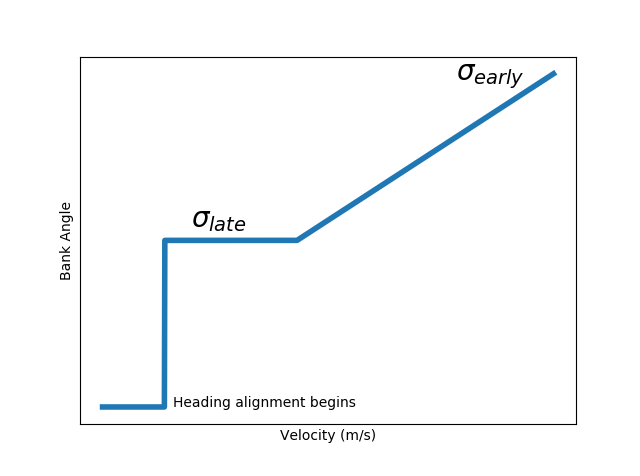
\includegraphics[width=4in]{MSLProfile.png}
		\caption{\bf{MSL's bank angle parametrization.}}
		\label{MSLParametrization}
	\end{figure*}
	\begin{figure*}
		\centering
		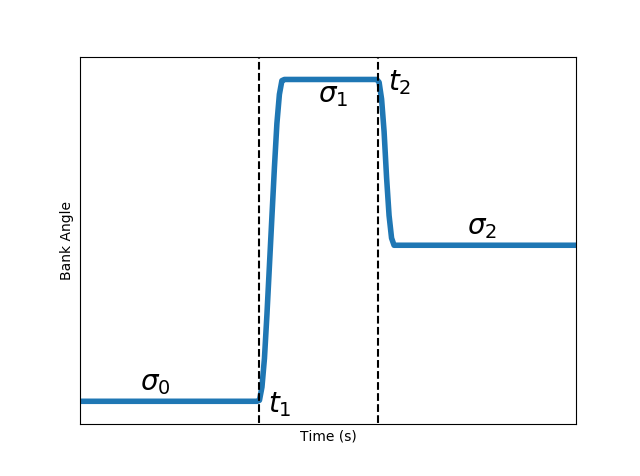
\includegraphics[width=4in]{BankAngleProfile.png}
		\caption{\bf{The proposed bank angle parametrization.}}
		\label{RefTrajParametrization}
	\end{figure*}
	
	\subsection{Entry Guidance}
	MSL's entry guidance consisted of three phases. The first was a pre-bank phase in which the vehicle flew a constant bank angle prior to entering the atmosphere. The phase ended when the drag acceleration exceeded 0.2 Earth g, and the range control phase began. Range control used a modified version of the Apollo shuttle guidance to predict the downrange flown and steer the bank angle to rectify range errors. The separate lateral logic referred to earlier consists of a velocity-dependent crossrange corridor in which the guidance commands a bank reversal whenever the onboard estimate of crossrange to target exceeds the corridor threshold. The final phase is heading alignment in which the vehicle is commanded to aim the vehicle toward the target point. This phase began at a fixed velocity which for MSL was 1100 m/s. The magnitude of the bank angle is saturated to 30$^\circ$ to ensure most of the lift generated is countering gravity to maintain adequate chute deployment altitude. Parachute deployment beginning terminal descent was initiated at a fixed Mach number of 2.
	
	The Apollo guidance adapted for MSL is essentially an LQR approach in which so-called "influence coefficients" are computed and used as velocity-varying gains for the feedback controller. These gains are computed on the ground and stored onboard the GNC flight computer. Rather than perform state feedback directly, the spacecraft states such as altitude and flight path angle are instead replaced by quantities that are better measured or estimated onboard, including aerodynamic drag and altitude rate. 
	
	The free parameters in this guidance approach consist of the pre-bank angle, the range control gain (sometimes referred to as the Overcontrol gain, or $ K_3 $), and the bank reversal deadbands. Additionally, the reference profile generated by the bank angle parametrization and the velocity at which heading alignment begins will also impact the results. The onboard estimates of drag and lift-to-drag ratio are each filtered with their own time constants.\cite{MSL_EDL_Overview_JPL}
		%Fisher and Bhattacharya use polynomial chaos expansions and direct optimal control to solve for an open loop control to steer systems with probabilistic parametric uncertainty.
		
%		The ultimate goal in controlling an uncertain system is to steer an entire distribution of states to some final distribution. Although it may be desirable to steer the entire distribution of states. 
		
	% Outline
	% Full stochastic optimal control problem - GNC strategy + reference traj
	% Conversion into stochastic NLP (via control parametrization based on optimal control techniques) then into deterministic NLP (based on QMC, PCE, STM, Unscented)
	\section{Entry Guidance as an Optimization Under Uncertainty Problem}
%	Consider the dynamics given by the deterministic ordinary differential equations. Due to uncertainty in the vehicle's initial state and parameters of the model, evolution of the trajectories is stochastic. Define the joint PDF of the uncertainty space $ \Delta $ and its support $supp(\Delta)\equiv\Omega$. By appending the uncertain model parameters to the state vector, all uncertainty can be lumped into the initial conditions without loss of generality and thus each realization of $x_0\in\Omega$ admits a deterministic solution $ x(t;x_0) $. 
	
	The goal is to design a reference trajectory and feedback controller that together constitute a guidance approach capable of steering the stochastic trajectory evolution to the target in expectation and with minimal variance. Thus we define the problem as finding the feedback control $u\equiv u(x,x_{Ref})$ that minimizes
	\begin{align}
		J = \mathbb{E}[(DR-DR_{Target})^2 + (CR-CR_{Target})^2]
	\end{align}
	subject to 
	\begin{align}
		&\dot{x} = f(x,u) \\
		&x_0 \in \Omega
	\end{align}
	
	To see that this cost function reduces both the error in expectation as well variance, define the horizontal error $e$ such that
		\begin{align}
		e^2(x_f) \equiv (DR-DR_{Target})^2 + (CR-CR_{Target})^2
		\end{align}
	and so $	J = \mathbb{E}[e^2]$. Let $\bar{e} = \mathbb{E}[e]$, and then by rearrangement of the definition of variance of a scalar random variable
		\begin{align}
		\mathbb{V}[e] = \mathbb{E}[e^2] - \bar{e}^2
		\end{align}
	we find that 
		\begin{align}
		J = \bar{e}^2 + \mathbb{V}[e].
		\end{align}
	Thus the cost function is an equal weighting of the square of the mean error and its variance. It is clear that $ J $ is a non-negative function and that a solution achieving the global optimum $ J=0 $ implies every trajectory is successfully driven to the targeted downrange and crossrange.
	
	\subsection{Sketch of the Algorithm}
	At the heart of the approach is the desire to optimize the reference data and controller parameters simultaneously. This is because an optimal reference profile combined with an optimized controller does not yield optimal performance. Given an initial PDF, use the mean initial state for reference computation and perform the following steps:
	\begin{enumerate}
		\item An outer optimization loop first selects the free parameters (e.g., bank angle profile parameters such the switching times $t_i,\;i=1:n$ and bank angles $\sigma_i,\;i=0:n$, as well as any free controller parameters)
		\item Integrate the reference trajectory forward to the final energy
		\item Compute the reference objective function value
		\item If $ J_{ref} < J_{threshold} $: store reference quantities (e.g., drag and its derivatives as functions of energy) and continue to next step;\\
		Else: return to the first step and select new parameters
		\item Integrate (preferably in parallel or vectorized manner) $ N $ trajectories using samples drawn from the initial PDF with closed-loop guidance using the selected parameters from step 1
		\item Optionally, if a metamodeling technique is used, construct a metamodel and evaluate it at $N_{meta}>> N$ points sampled from the initial PDF
%		\item Integrate (preferably in parallel or vectorized manner) $ N_{PCE} $ trajectories using samples drawn from the initial PDF with closed-loop guidance using the selected parameters from step 1
%		\item Construct a polynomial chaos expansion from these $ N_{PCE} $ evaluated trajectories
%		\item Evaluate the PCE model at $ N $ points (typically $N_{PCE}\ll N $) sampled from the initial PDF
		\item Determine the final state $x^i_{f}$ of each trajectory ($i\in \mathbb{N}$, $i<N$ for sampling or $i < N_{meta}$ for metamodel version) by applying the parachute deployment conditions
		\item Evaluate the closed-loop cost estimate by taking the expectation over all trajectories
	\end{enumerate}
		
		

	\subsection{Reference Trajectory Design}
	In order to use a tracking controller to guide the vehicle, a suitable reference trajectory is required. The features of a desirable reference trajectory include high performance in the nominal scenario while leaving appropriate margin for the controller to compensate stochastic uncertainty. Naturally standard optimal control techniques can be used to solve for a trajectory that extremizes some feature(s) such as maximizing final altitude at parachute deployment, or minimizing propellant required to land via retropropulsion technology. It does not offer a clear method to determine how much margin is sufficient for the controller (indeed, the optimization knows nothing about the controller to be used, and different controllers will in general require different amounts of control margin). There is a well-known tradeoff between optimality and robustness. In a system with limited control authority, the optimal solution will use all available control and typically ad hoc methods are used to choose the margins. If more margin than is needed is allocated, performance of the reference trajectory (and of the corresponding mean trajectory of the stochastic system) will deteriorate. Note that the reference trajectory uses $ \mathbb{E}[x_0] $ and can therefore be shown to be a first order approximation to the expected trajectory by Taylor expansion.
	
	The deterministic cost used in generating an optimal reference trajectory is given by 
	\begin{align}
	J_{ref} = -h(V_f) + |CR(V_f)| + \kappa|DR(V_f)-DR^*| \label{eq_cost_deterministic}
	\end{align}
	which seeks to maximize final altitude while reaching approximately zero crossrange at a specified final velocity. Setting $\kappa=1$ seeks a solution that also satisfies a downrange requirement $DR(V_f)=DR^*$ while $\kappa=0$ leads to an optimal solution over all reachable downrange distances. 
	
	\textbf{Talk about the threshold step.}
			
	\subsection{Closed Loop Performance Evaluation}		
	In addition to the reference trajectory, the controller parameters must also be chosen judiciously to maximize performance. The cost function used depends on the uncertainty space $ \Delta $ and its support $supp(\Delta)\equiv\Omega$.		
			
	In contrast to the open loop formulation employed by Ref.~\cite{RSOptimalControl} where a single control trajectory aims to steer an entire tube of trajectories, we consider the closed loop formulation where both the reference (which in some sense constitutes the open loop portion of the control) and the controller parameters (for an a priori chosen controller design) are optimized. (Part of the optimization could even be selecting which controller is best!)		
	
	Three approaches to the forward uncertainty quantification have been investigated: linear sensitivity (aka state-transition method), quasi-Monte Carlo methods, and polynomial chaos expansions.  
			
	\subsection{Entry Termination Logic}
	The logic which decides when the entry phase ends is instrumental to good horizontal performance while ensuring the vehicle is in an appropriate state to deploy a parachute or otherwise initiate a final descent phase. Compare the results of a fixed energy trigger, in which all trajectories end at the same energy as the reference trajectory, and the combined parachute-range control logic as summarized in Figure \textbf{Put a figure}. \textbf{Show the two sets of final states (h-v, lat-lon)}
	
	Unfortunately, this logic is not differentiable, and thus precludes the use of polynomial chaos to expand the cost function directly. Instead, the state trajectories themselves are expanded. This allows the non-smooth trigger to be incorporated while still leveraging the PCE models. The downside is that considerably more models must be constructed (one for each state variable used in the cost function, times a fraction of the total number of timesteps taken during integration). The PCE models are then sampled extensively (because the cost to do so is low relative to the cost of constructing the models) and the trigger logic is applied to each trajectory to find its final state. Then, the expectation of the cost is simply estimated as $\mathbb{E}[J]\approxeq\frac{1}{N}\sum_{i=1}^{N}J(x_f^i)$. 
			
			
	\subsection{Global Optimization}
	The resulting optimization problem may be solved by a number of methods and is not the intended focus here. Both differential evolution and particle swarm optimization have been used to successfully solve this problem. Convergence in both cases can be improved by seeding the initial population with appropriate guesses. 	
	
	\section{Uncertain Optimal Control via Continuation}
	
	Many deterministic optimal control problems can be solved via existing methods, both direct and indirect. When the dynamics are uncertain, due to variations in system parameters or initial state, the problem becomes more difficult. Ref.~\cite{RSOptimalControl} presents an extension of the pseudospectral methodology for numerical optimal control to the uncertain case. Ref.~\cite{UncertainOptimalControl} also used a direct method to solve sample average approximations to the stochastic problem. In contrast to these direct methods, we propose an indirect method based on Pontryagin's maximum principle, continuation, and sample average approximations. 
	
	Consider systems with dynamics given by deterministic ordinary differential equations. Due to uncertainty in the system's initial state and parameters of the model, evolution of the trajectories is stochastic. Let the joint PDF of the uncertainty space be $ \Delta $ and its support $\mathrm{supp}(\Delta)\equiv\Omega$, and denote by $\mathbb{E}[\cdot]$ the expectation taken with respect to $\Delta$. Both $\Delta$ and $\Omega$ vary with time. Let $\tau=t/t_f$, and define $(\cdot)'=\dfrac{\partial}{\partial\tau}$. By appending the uncertain model parameters to the state vector, all uncertainty can be lumped into the initial conditions without loss of generality and thus each realization of $x_0\in\Omega(0)$ admits a deterministic solution $ x(\tau;x_0)$ (in general the dependence on $ x_0 $ is suppressed). Thus the state $x: [0,1]\times\Omega\mapsto\mathbb{R}^n$ and control $u: [0,1]\mapsto U\subseteq\mathbb{R}^m$. The uncertain optimal control problem we seek to solve minimizes the expectation of a functional in Mayer form subject to deterministic dynamics $f: \mathbb{R}^n \times U \mapsto \mathbb{R}^n$ with stochastic initial conditions, control constraints, and a free final time $t_f$:
	\begin{align}
	\min_{u\in U} \;&J = \mathbb{E}[\varphi(x(1))] \label{eq_generic_uncertain_mayer}  \\
		&x' = f(x,u)\cdot t_f \\
		&x(0)= x_0 \in \Omega(0) %\\
		%&u(t,x) \in U
	\end{align}	
	Consider an N-sample average approximation to Eq.~\ref{eq_generic_uncertain_mayer} given by		
	\begin{align}
	J_N = \frac{1}{N}\sum_{i=1}^{N}\varphi(x_i(1)). \label{eq_saa_mayer}
	\end{align}	
	Ref.~\cite{UncertainOptimalControl} showed that under appropriate conditions Eq.~\ref{eq_saa_mayer} produces a meaningful approximation to Eq.~\ref{eq_generic_uncertain_mayer}. 
	
	For each $x_0 \in \Omega(0)$, there is an associated costate $\lambda(\tau, x_0)$ such that the Hamiltonian is given by $H(\tau, x_0) = f\cdot\lambda$, the costates satisfy
	\begin{align}
	\dot{\lambda} = -\nabla_xH
	\end{align} 
	and the optimal control is given by (Ref.~\cite{RSOptimalControl})
	\begin{align}
	u^*(t) = \arg\min_{u\in U}\mathbb{E}[H] \label{eq_uncertain_optimal_control}
	\end{align}
	
	An N-sample average approximation to the expected Hamiltonian may also be made
	\begin{align}
		H_N(\tau) = \frac{1}{N}\sum_{i=1}^{N}H(\tau,x_i(0)). \label{eq_saa_hamil}
	\end{align}	
	\textbf{Remark.} \textit{The uncertain scenario is significantly more difficult to solve via indirect method because we seek a single control function to steer the entire tube of trajectories, i.e. the optimal control minimizes the expected Hamiltonian at each point in time. In the deterministic case, the control can be computed from the costates given a guess at the initial costate values. In the uncertain case, the initial guess of costate values in now N times as large. Fortunately, via a homotopy method we can exploit nearness of solutions.}	
		
		
	In the case that $\Delta$ is a Dirac distribution supported at some nominal value $x_0$ then the uncertain problem reduces to a standard optimal control problem. This inspires the idea to define a homotopy between the standard OCP and the uncertain OCP. The only requirement is that the PDF may be sampled from. 
	
%	This requires parametrization of $\Delta$ by a factor $\epsilon\in[0,1]$ such that $\epsilon=0\implies\mathrm{diam}(\Omega)=0$ and $\epsilon=1\implies \Delta=\Delta_{des}$. For common distributions such as Normal, Uniform, Beta the parametrization is simple including multivariate cases. For example, a normal distribution with mean $ m $ and covariance $ P $ is parametrized simply as $ \mathcal{N}(m,\,\epsilon P) $. For a variable uniformly distributed between lower bound $ L $ and upper bound $ U $, let $ m = \frac{(L+U)}{2}$ and $b = \frac{(U-L)}{2}$, then the distribution may be parametrized $ \mathcal{U}(m-\epsilon b,\, m+\epsilon b ) $ 
	
	\begin{thebibliography}{1}
%		\bibitem{brockett2012}
%		R. W. Brockett. ``Notes on the control of the Liouville equation'' In P. Cannarsa and J. M.
%		Coron, editors, Control of Partial Differential Equations, pages 101-129. Springer,
%			Berlin-Heidelberg, 2012.
		

		\bibitem{MSL_EDL_Overview_JPL}
		A.D. Steltzner, P.D. Burkhart, et. al, ``Mars Science Laboratory Entry, Descent, and Landing System Overview," 2010.
				
		\bibitem{MSL_EG_Mendeck_Craig}
		G.F. Mendeck, and L.E. Craig, ``Entry Guidance for the 2011 Mars Science Laboratory Mission," AIAA, 2010.
		
		\bibitem{High Elevation Landing}
		G. Duan, A. Bombelli, J. Benito, and K.D. Mease, ``High Elevation Planner for Mars Entry"
		
		\bibitem{RangeTriggerWay}
		D. Way, "On the use of a Range Trigger for the Mars Science Laboratory Entry Descent and Landing"
		
		\bibitem{RSOptimalControl}
		I.M. Ross, R.J. Proulx, M. Karpenko, and Q. Gong, ``Riemann-Stieltjes Optimal Control Problems for Uncertain Dynamic Systems," AIAA Journal of Guidance Control and Dynamics, 2015.
		
		\bibitem{UncertainOptimalControl}
		C. Phelps, J.O. Royset, and Q. Gong, ``Optimal Control of Uncertain Systems Using Sample Average Approximations," SIAM Journal on Control and Optimization, 2016.
	\end{thebibliography}
\end{document}